\chapter{Time Management}
\thispagestyle{fancy}
This chapter should help other students guessing the amount of work that is 
involved in writing a refactoring semester thesis.

\section{Time Budget}
The extent of work expected for a semester thesis at HSR is 8 ECTS which 
corresponds to an effort of 240 hours per person. Issues were created after 
the meetings on Thursday and an amount of time was guessed for them. 

\section{What the Charts are Saying}
These charts and tables illustrate the workload by week and by topic:

\begin{figure}[h]
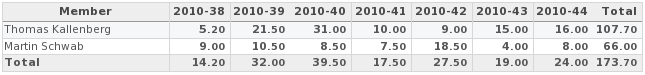
\includegraphics[width=1\textwidth]{images/timetable1.png}
\caption{Working hours of the team members by weeks from beginning of the
project to 11th of November}
\label{timetable1}
\end{figure}

\begin{figure}[h]
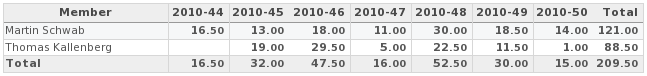
\includegraphics[width=1\textwidth]{images/timetable2.png}
\caption{Working hours of the team members by weeks from 11th November to 23rd
of December}
\label{timetable2}
\end{figure}

\section{What the Team is Saying}
Charts are generated out of numbers which have been typed in by humans. There 
has been a time between week eight and ten where time tracking was abandoned and 
added three weeks later. Also, there were a lot of discussions that could not 
have been assigned to a specific issue. Not every minute was tracked, so be 
aware that the actual spent time was about ten percent above the reported time.
